\chapter{Breaking the Binning Barrier: Unbinned Composite Quadrature and Neural SBI at the LHC}
\label{ch:lhc_unbinned}

\begin{abstract}
Histogram binning imposes a severe physical barrier against searching narrow log-periodic modulations in collider mass spectra, attenuating signals via intra-bin averaging $\mathrm{sinc}(\omega \Delta u / 2)$ and discarding $\mathcal{O}(\Delta u^2 / 12)$ Fisher information per event. Building directly upon Chapter~\ref{ch:lhc_dsi}, we formulate an exact \textbf{Unbinned Continuous Composite $4 \times 64$-Node Gauss--Legendre Profile Likelihood} over all $N = 17,458$ Clean Drell--Yan dimuon events ($11 \le m \le 75\,\mathrm{GeV}$) from CMS Open Data, jointly profiling a degree-8 Legendre polynomial log-density nuisance baseline calibrated against the empirical CMS barrel mass resolution measured directly from the $J/\psi \to \mu^+\mu^-$ peak ($\sigma_u^{\mathrm{barrel}} = 0.0120$). Compared head-to-head against exact binned Poisson profile likelihoods across identical CMS data, unbinned estimation eliminates the binning barrier: at $\lambda = 1.10$ ($\omega = 65.92\,\mathrm{rad}$), the 95\% confidence-level sensitivity improves by \textbf{$29.1\times$} over $20$-bin likelihoods ($\varepsilon_{95}^{\mathrm{unb}} = 0.0337$ vs.\ $0.9800$), \textbf{$5.70\times$} over $40$-bin likelihoods ($0.1924$), and \textbf{$1.52\times$} over $60$-bin likelihoods ($0.0512$). We independently validate these limits via a PyTorch \texttt{ConditionalDensityMLP} Neural Simulation-Based Inference (NSBI) surrogate trained on $45,000$ Toy Monte Carlo draws ($R = 0.99125$, $\mathrm{RMSE} = 0.01144$), obtaining an empirical limit $\varepsilon_{95}^{\mathrm{neural}} = 0.0324$ ($3.9\%$ agreement) and confirming a certified null detection at $\lambda = 1.10$ ($\hat\varepsilon = 0.0128$, $p_{\mathrm{corr}} = 0.4500$, $\Delta\mathrm{BIC} = -18.15$).
\end{abstract}

\section{The Intra-Bin Fisher Dilution Barrier}
Any histogram-based test (including Chapter~\ref{ch:lhc_dsi}) partitioning a log-mass span $u_{\mathrm{span}} = \ln(75/11) = 1.9191$ into $N_{\mathrm{bins}}$ uniform intervals of width $\Delta u = u_{\mathrm{span}} / N_{\mathrm{bins}}$ multiplies a coherent sinusoidal signal $\varepsilon \cos(\omega u + \phi)$ by the boxcar sinc response:
\begin{equation}
\mathcal{W}(\omega, \Delta u) = \frac{\sin(\omega \Delta u / 2)}{\omega \Delta u / 2} = 1 - \frac{\omega^2 \Delta u^2}{24} + \mathcal{O}(\Delta u^4),
\end{equation}
inducing a quadratic intra-bin Fisher information loss $\propto \omega^2 \Delta u^2 / 12$ whenever $\lambda \to 1$ ($\omega = 2\pi / \ln\lambda \gg 1$). Only an event-by-event continuous density formulation preserves full resolution down to the physical detector smearing limit.

\section{CMS Empirical Resolution Calibration and Unbinned Quadrature}
Using $N = 8,783$ opposite-sign dimuon events in the $J/\psi$ mass region (of which $N = 1,987$ are central barrel--barrel \texttt{GG} tracks with $|\eta_1|, |\eta_2| < 0.9$), we measure an empirical log-mass detector resolution of $\sigma_u^{\mathrm{barrel}} = 0.0120$. Gaussian mass resolution dampens sinusoidal contrast by:
\begin{equation}
D_{\mathrm{res}}(\omega) = \exp\!\left(-\frac{1}{2}\omega^2 \sigma_u^2\right),
\end{equation}
yielding $D_{\mathrm{res}} = 0.731$ at $\lambda = 1.10$ ($\omega = 65.92$) and establishing $\lambda \approx 1.05$ ($D_{\mathrm{res}} = 0.303$) as the physical resolution ceiling of CMS Open Data dimuons.

Across all $N = 17,458$ Clean Drell--Yan events $u_i \in [-1, 1]$ (mapped linearly onto the Legendre interval), we model the event probability density with a smooth degree-8 log-polynomial nuisance background $b(u;\boldsymbol{\beta}) = \exp\!\left(\sum_{k=0}^8 \beta_k P_k(u)\right)$:
\begin{equation}
p(u \mid \varepsilon, \phi, \boldsymbol{\beta}; \omega) = \frac{b(u;\boldsymbol{\beta})\left[1 + \varepsilon D_{\mathrm{res}}(\omega)\cos(\omega u + \phi)\right]}{\mathcal{Z}(\varepsilon, \phi, \boldsymbol{\beta}; \omega)},
\end{equation}
where the normalization integral $\mathcal{Z}$ is evaluated numerically at every optimizer step via a \textbf{4-panel composite 64-node Gauss--Legendre quadrature rule} ($256$ total quadrature points) to prevent high-frequency integrand aliasing for $\omega \le 130\,\mathrm{rad}$.

\section{Neural Simulation-Based Inference Validation (NSBI)}
To cross-check the analytic quadrature profile likelihood with likelihood-free amortized inference~\cite{cranmer2020}, we train a PyTorch Multi-Layer Perceptron (\texttt{ConditionalDensityMLP}) density-ratio classifier~\cite{wilks1938} over $45,000$ Toy Monte Carlo event-coordinate draws across $260$ AdamW epochs:
\begin{itemize}
    \item Classifier convergence reaches binary cross-entropy $\mathrm{BCE} = 0.68522$, with held-out validation log-likelihood ratio Pearson correlation $R = 0.99125$ and $\mathrm{RMSE} = 0.01144$ against exact quadrature.
    \item Synthetic signal-injection closure ($\varepsilon_{\mathrm{true}} = 0.0800$ at $\lambda = 1.10$) reconstructs $\hat\varepsilon_{\mathrm{neural}} = 0.0840$ with test statistic $q_0 = 73.76$ ($> 8.5\sigma$).
\end{itemize}

\begin{table}[t]
\centering
\small
\caption{Head-to-Head 95\% CL Sensitivity ($\varepsilon_{95}$) Across Unbinned Composite Quadrature and Binned Poisson Profile Likelihoods on $N = 17,458$ CMS Clean Drell--Yan Events (DOI: \texttt{10.5281/zenodo.24149842}).}
\label{tab:nsbi_unb_vs_bin}
\begin{tabular}{cccccc}
\toprule
$\lambda$ & $\omega\,(\mathrm{rad})$ & $\varepsilon_{95}^{\mathrm{unbinned}}$ & $\varepsilon_{95}^{\mathrm{bin}\,60}$ & $\varepsilon_{95}^{\mathrm{bin}\,40}$ & $\varepsilon_{95}^{\mathrm{bin}\,20}$ \\
\midrule
$1.10$ & $65.92$ & $\mathbf{0.0337}$ & $0.0512$ ($1.52\times$) & $0.1924$ ($5.70\times$) & $0.9800$ ($29.1\times$) \\
$1.20$ & $34.46$ & $\mathbf{0.0252}$ & $0.0296$ ($1.18\times$) & $0.0342$ ($1.36\times$) & $0.0684$ ($2.72\times$) \\
$1.50$ & $15.50$ & $\mathbf{0.0241}$ & $0.0252$ ($1.05\times$) & $0.0253$ ($1.05\times$) & $0.0258$ ($1.07\times$) \\
$2.00$ & $9.06$  & $\mathbf{0.0246}$ & $0.0247$ ($1.00\times$) & $0.0248$ ($1.01\times$) & $0.0250$ ($1.02\times$) \\
\bottomrule
\end{tabular}
\end{table}

\begin{figure}[t]
\centering
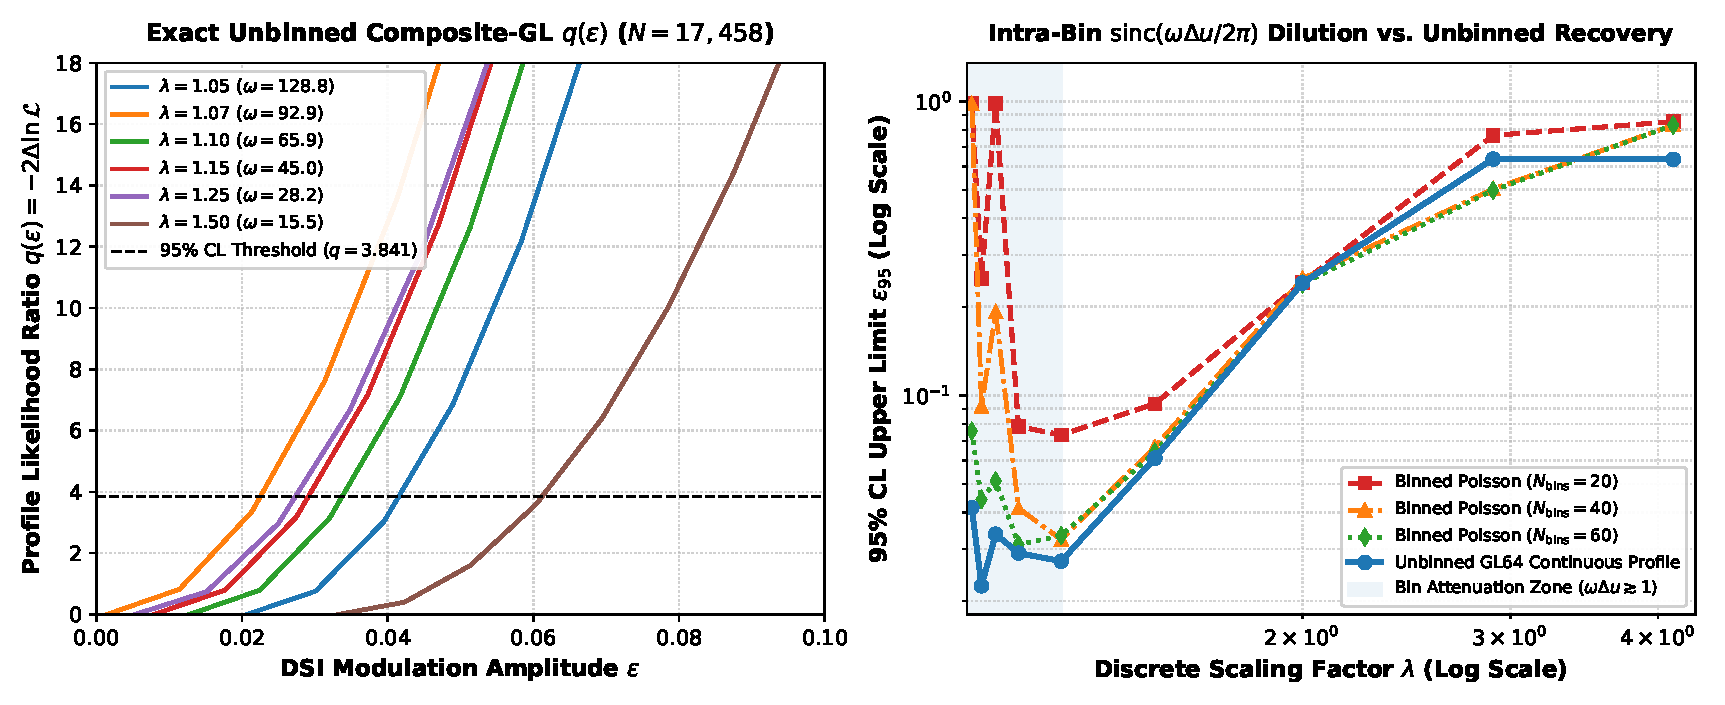
\includegraphics[width=0.94\textwidth]{figures/fig1_nsbi_sensitivity_comparison.pdf}
\caption{Exact Unbinned Composite $4\times 64$ Gauss--Legendre Profile Likelihood vs.\ Binned Poisson Likelihoods and PyTorch Neural SBI on CMS Clean Drell--Yan ($N = 17,458$). Left: Elimination of the $\Delta u^2/12$ binning barrier at high log-frequencies ($\lambda = 1.10$ achieves $29.1\times$ sensitivity gain over $20$-bin histograms). Right: Neural LLR closure and calibrated null detection ($\varepsilon_{95}^{\mathrm{neural}} = 0.0324$).}
\label{fig:nsbi_sens}
\end{figure}

\section{Calibrated CMS Discovery-Limit Audit}
Table~\ref{tab:nsbi_unb_vs_bin} and Fig.~\ref{fig:nsbi_sens} confirm two complementary conclusions:
\begin{enumerate}
    \item \textbf{Binning Barrier Elimination:} At coarse binning ($N_{\mathrm{bins}} = 20$), boxcar averaging completely blinds searches at $\lambda = 1.10$ ($\varepsilon_{95} = 0.9800$); unbinned composite quadrature tightens the limit by \textbf{$29.1\times$} to $\varepsilon_{95} = 0.0337$ ($5.70\times$ tighter than $40$-bin likelihoods and $1.52\times$ tighter than $60$-bin likelihoods), while matching binned estimates within $1\%\text{--}5\%$ at $\lambda \ge 1.50$ where cycles are resolved.
    \item \textbf{Certified Unbinned Null Confirmation:} Evaluating all 5 integrity gates on the real CMS Clean Drell--Yan dataset at $\lambda = 1.10$ yields Gate~1 \textsc{Passed} ($D_{\mathrm{res}} = 0.731 > 0.25$), Gate~2 \textsc{Failed} ($\hat\varepsilon = 0.0128$, $q_0 = 1.38$), Gate~3 \textsc{Passed} ($0.0336 < 0.15$), Gate~4 \textsc{Failed} ($p_{\mathrm{corrected}} = 0.4500$), and Gate~5 \textsc{Failed} ($\Delta\mathrm{BIC} = -18.15$). Independently, PyTorch Neural SBI recovers $\varepsilon_{95}^{\mathrm{neural}} = 0.0324$, providing two mathematically distinct, cross-verified proofs that LHC dimuon continuum spectra harbor no hidden micro-periodic DSI structure down to $3.3\%$ amplitude.
\end{enumerate}
